\documentclass{article}
\usepackage{kotex}
\usepackage{graphicx}
\usepackage{amsmath}
\renewcommand{\figurename}{그림}
\usepackage[labelsep=period]{caption}
\usepackage{subfigure}
\setcounter{figure}{2}
\setcounter{equation}{4}

\begin{document}
	\begin{figure}[h]
		\centering
		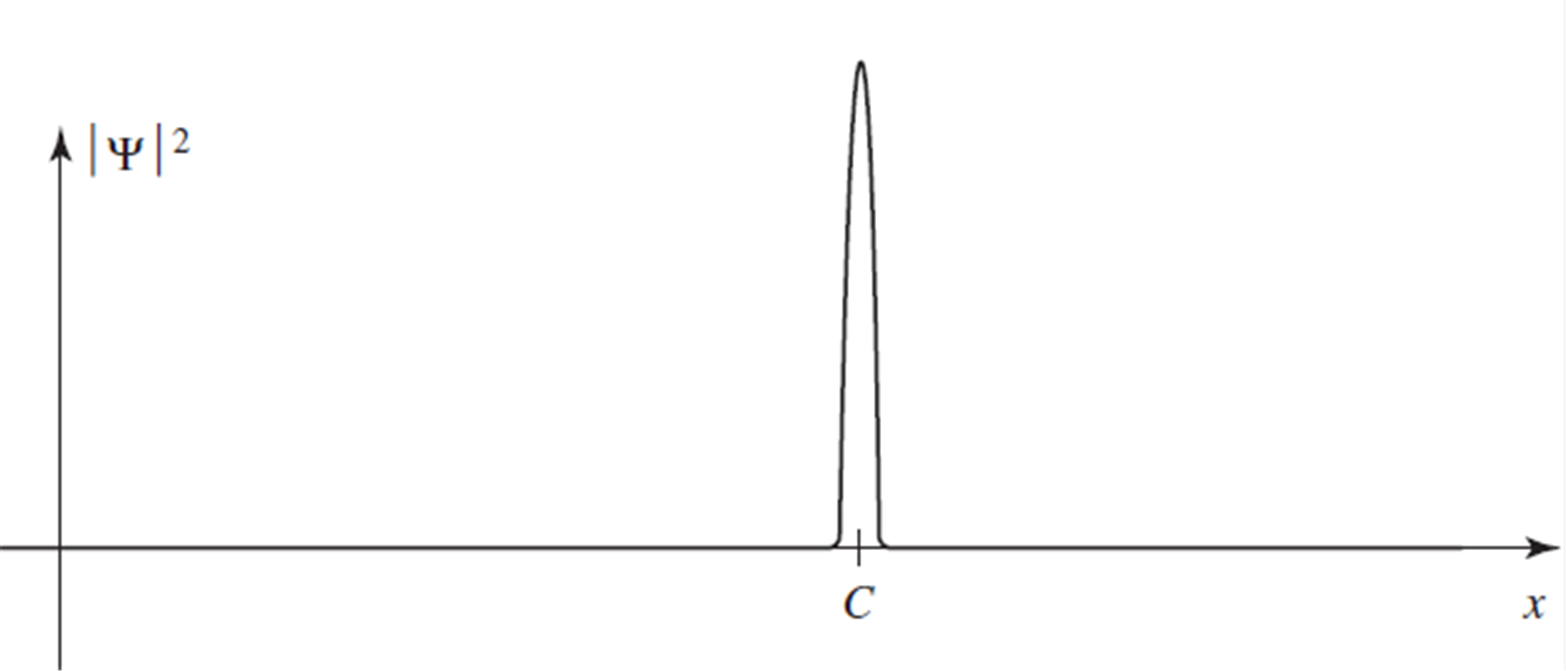
\includegraphics[width=0.5\textwidth]{wave_function.png}
		\caption{파동 함수}
		\label{fig:wave_function}
	\end{figure}
	그림 \ref{fig:wave_function}은 파동 함수의 모습이다. 여기서 규격화 조건은 식 \eqref{eq:normalization}이다\cite{griffiths2018}.
	\begin{equation}
		\int_{-\infty}^{\infty} |\Psi|^2 dx = 1
		\label{eq:normalization}
	\end{equation}
	
	
\begin{thebibliography}{99}
	\bibitem{gac2020} Gemelli Against COVID-19 Post-Acute Care Study Group. (2020). Post-COVID-19 global health strategies: the need for an interdisciplinary approach. Aging Clinical and Experimental Research, 1.
	\bibitem{tic2020} Team IHME COVID, Reiner, R. C., Barber, R. M., \& Collins, J. K. (2020). Modeling COVID-19 scenarios for the United States. Nature medicine.
	\bibitem{griffiths2018} David J. Griffiths. (2018). Introduction to Quantum Mechanics
\end{thebibliography}
\end{document}